\subsection{Statistical Model Selection via Argumentation}
\label{sub:statistical_model_selection}
The foundation of this MSc Project is the paper \cite{sassoon2014}. 
The goal of this project is to use Argumentation Theory for Statistical Model Selection in mostly clinical environments. The demand into systems that support clinicians in the analysis of this data in their day-to-day practice is extending (because of increasing availability, growing size of datasets available for clinicians, and raising awareness on evidence based decision making extend). In the following section a short summary on the paper will be given. 

To overcome the issue of clinicians analysing data and models on their compatibility \cite{sassoon2014} proposes an approach of an intelligent model selection system which is capable of suggesting appropriate model(s) to a clinician during the design stage of a study, taking in account the research question, the clinical data and any external relevant input and preferences. In addition this system should be able to support its decision by providing the argumentation for and against a model to the user. As clinicians might not always be qualified to perform the statistical analysis required for their research question, the process of designing models, specifying its requirements and providing the arguments for or agains these models should be separated from the actual design process and be done by a statistician. The statistician is thereby  charge of understanding the data in the context of the research question and provide arguments that are able to recommend the best suited statistical analysis for a particular research question. 

Furthermore  Sassoon \textit{et al.} \cite{sassoon2014} addresses the problem of defeasible knowledge, as the (counter)arguments for a model are often contradicting and the system, the clinician and the statistician might have some preferences for one or the other model. Therefore Sassoon \textit{et al.} propose to split the problem into two parts (i) a (defeasible) \textit{knowledge base} that contains the statistical model definitions, the objectives and assumptions of a model; (ii) \textit{argumentation schemes} to guide the model selection process and to represent expressed preferences.

The \textit{knowledge base} is used to instantiate the \textit{argumentation schemes}. The knowledge base itself defines how research objectives can be achieved through different statistical models considering their given assumptions. \textit{Research objectives} are defined as different 'families' of analysis (e.g. survival analysis or categorical outcome variable analysis).


\glsreset{SKB}
\subsubsection*{Statistical Knowledge Base}


The \gls{SKB} consists of objectives $O=\{o_1, ..., o_u\}$ (different types of research questions), models $M=\{m_1, ..., m_v\}$ and assumptions $A = \{a_1, ..., a_w\}$. Models represent statistical analysis techniques employable to answer a research question. Assumptions are conditions that ought to be met to employ a model.

\begin{definition}
	Let $R_{OM}: O \times M$ be a m:n\footnote{Each objective can be achieved by one or more models, each model can answer one or more objectives.}-relationship such that $(o_i, m_j)\in R_{OM}$ implies objective $o_i$ can be achieved by means of model $m_j$. 
\end{definition}

\begin{definition}
	Let $R_{MA}: M \times A$ be relation between models and their assumptions. $(m_i, a_j)\in R_{MA}$ implies  the model $m_i$ requires the assumption $a_j$ to be true to be applicable. Let $A(m_i) = \{a_j | (m_i, a_j) \in R_{MA}\}$ be the set of assumptions of $m_i$.
\end{definition}

As it will not always be possible to find a model where all assumptions are met, it will be necessary to apply a model even when there are some violations regarding the assumptions. Hence we need to specify whether an assumption $a_j$ is \textit{critical} to a model. If a critical assumption doesn't hold its model must not be applied under any circumstances.

\begin{definition}
Let $C \subset R_{MA}$ be the set of critical assumptions. To apply a model $m_i$ all critical assumptions $A_c(m_i) = \{a_j | (m_i, a_j) \in C\}$ must be met.
\end{definition}

Each \textit{assumption} will be either specified as a specific property of the data set (assessed by applying tests on the data set) or as a characteristic of the population of interest or the way in which the data set was collected from that population (relying on the expertise of a domain expert). Sassoon proposes a partitioning of all assumptions: $A_t$ denotes the set of tests (and apply a test on the available data set). $A_q$ denotes the set of queries (and will be assessed by asking the clinician for an opinion). Lets define $A_t(m_i)= \{a_j| (m_i, a_j) \in A_t\}$ and $A_q(m_i)= \{a_j| (m_i, a_j) \in A_q\}$. Note that critical assumptions can be in either $A_t$ or $A_q$: $C \subset R_{MA} = A_q \cup A_t, ~A_q \cup A_t = \emptyset$. 

The \autoref{fig:skb_example} shows the structure between \textit{objectives}, \textit{models} and \textit{assumptions} in a small example. The assumptions $\{a_1, a_2, a_3\} \in A_t$ are based on the provided data set, $\{a_3, a_5\} \in A_q$ are based on the domain expertise. Objectives $\{o_1, o_2\}$ can  be achieved by the possible model $m_1$, $o_3$ can only be achieved by $m_3$. Note that $m_3$ is still a possible model although the non critical assumption $a_4$ doesn't hold.

\begin{figure}[h]
\centering
\begin{tikzpicture}[->,>=stealth',shorten >=1pt,auto,node distance=1cm,
                    thick]

  \node[main node] (o1) {$o_1$};
  \node[main node] (o2) [below of=o1] {$o_2$};
  \node[main node] (o3) [below of=o2] {$o_3$};

  \node[main node,n_fill_green] (m1) [right= 1.5cm of o1] {$m_1$};
  \node[main node,n_fill_red] (m2) [below of=m1] {$m_2$};
  \node[main node,n_fill_green] (m3) [below of=m2] {$m_3$};

  \node[main node, double,n_fill_red] (a2) [right= 1.5cm of m1] {$a_2$};  
  \node[main node,n_fill_green] (a1) [above of=a2] {$a_1$};
  \node[main node, double,n_fill_green] (a3) [below of=a2] {$a_3$};
  \node[main node,n_fill_red] (a4) [below of=a3] {$a_4$};
  \node[main node, double,n_fill_green] (a5) [below of=a4] {$a_5$};
  
  \node (DB) [cylinder, shape border rotate=90,draw,minimum height=2cm,minimum width=1.3cm, fill=gray!10][right= 3cm of a2]{DB};
  \node (T) [draw=black,fill=gray!10,cloud,font=\fontfamily{ppl}\fontsize{1cm}{1.5cm}\selectfont][right= 3cm of a4]{?};
  
  \path[every node/.style={font=\sffamily\small}]
    (a1) edge [] node [left] {} (m1)
         edge [] node [left] {} (m2)
    (a2) edge [] node [left] {} (m2)
    (a3) edge [] node [left] {} (m2)
    (a4) edge [] node [left] {} (m2)
         edge [dashed] node [left] {} (m3)
         edge [] node [left] {} (m3)
    (a5) edge [] node [left] {} (m3)
    (m1) edge [] node [left] {} (o1)
         edge [] node [left] {} (o2)
	(m2) edge [] node [left] {} (o1)
	     edge [] node [left] {} (o2)
	(m3) edge [] node [left] {} (o3)
	(DB) edge [] node [left] {} (a1)
         edge [] node [left] {} (a2)
         edge [] node [left] {} (a4)
         edge [] node [left] {} (a1)
    (T)  edge [] node [left] {} (a3)
         edge [] node [left] {} (a5)
    ;
\end{tikzpicture}
\caption{Example of a \gls{SKB}. Double circled assumptions represent critical assumptions. Green coloured assumptions hold while red coloured assumptions do not hold. Green coloured models are the possible models.}
\label{fig:skb_example}
\end{figure}



\subsubsection*{Different Processes to instantiate Arguments from the Knowledge Base}

To achieve an objective $o_c$ (which has been selected by the clinician) a number of models $m_i$ might be possible providing their critical assumptions $A_c(m_i)$ are met. The process of instantiating the arguments can be seen in AS\autoref{as:1}. To elaborate one model $m_i$ which is preferred over the other possible models we define a Model Preference as depicted in AS\ref{as:2}.

\begin{AS}[h]
\centering
	\caption{Constructed argument for a Possible Model.\label{as:1}}
	\fbox{\begin{minipage}{0.7\textwidth}
	\begin{itemize}
		\item Model $m_i$ achieves objective $o_c$.
		\item The data set meets the set of assumptions $A_t' = A_t(m_i)$.
		\item The research project meets the set of assumptions $A_q' = A_q(m_i)$.
		\item $A_c(m_i) \subseteq A_t' \cup A_q'$.
	\end{itemize}
	\rule{\textwidth}{0.5pt}\\
	$~~~~\Rightarrow$  $m_i$ is a possible model for the research question $o_c$.
	\end{minipage}}
\end{AS}

Depending on the purposes of models and on the reasons for preferring one model over another there are different ways of implementing $(\ast)$ in the generic definition provided in AS\ref{as:2}. These different reasons to prefer one model over another depend on the context and on the application, however \cite{sassoon2014} proposes different approaches to express the preference of one model over another.  

\todo{remove AS2 and change to context domain}
\begin{AS}[h]
\centering
	\caption{Argument for a Model Preference between two possible models.\label{as:2} }
\fbox{\begin{minipage}{0.7\textwidth}
	\begin{itemize}
		\item $m_i$ is a possible model.
		\item $m_j$ is a possible model.
		\item there is some reason to prefer $m_i$ over $m_j$ ($\ast$)
	\end{itemize}
	\rule{\textwidth}{0.5pt}\\
	$~~~~\Rightarrow$  $m_i$ is preferred over $m_j$.
	\end{minipage}}

\end{AS}

To express the preferences for one model over another, Sassoon \textit{et al.} \cite{sassoon2016} propose to use \gls{EAF} \cite{Modgil2009} in combination with \gls{PAF} \cite{amgoud,amgoud2000} approaches, both been presented earlier in this paper. These modifications enable argumentation on preferences which are encapsulated as arguments, therefore we will be able to consider conflicting preferences in our system and ensure scalability and express orders of importance between statistical reasons to prefer one model over another and clinician's preferences in specific contexts.

\todo{Context domain approach as presented in isabels latest paper}
\todo{Source by isabel for pic below}
\begin{figure}[h]

\centering
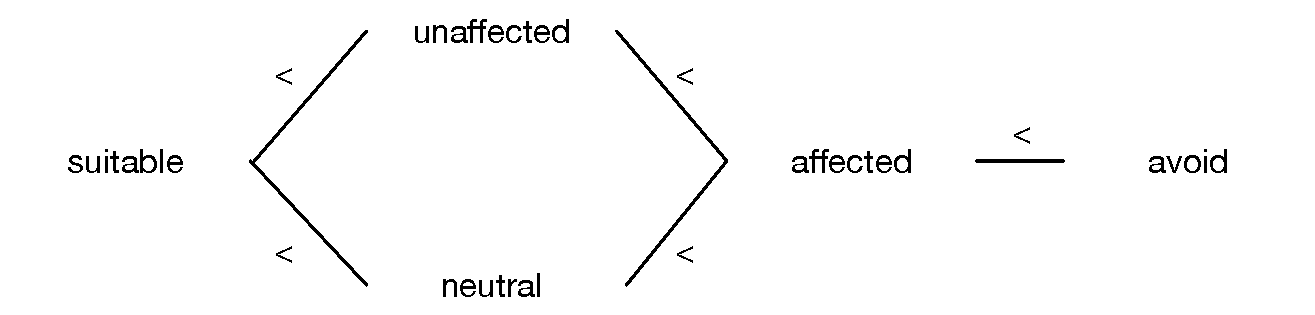
\includegraphics[width=0.8\textwidth]{figures/order_context_domain}
\caption{Order of different results in context domains }
\end{figure}

